\documentclass[xcolor={dvipsnames,table}]{beamer}
\usepackage{tikz}                   
\usetikzlibrary{shadows}
\usetheme{Dresden}
\usepackage[utf8]{inputenc}
\usepackage{polski}
\setbeamertemplate{blocks}[rounded][shadow=true]
\setbeamertemplate{footline}[frame number]
\usepackage{booktabs}
\usepackage{listings}
\usepackage{color}
 
\definecolor{codegreen}{rgb}{0,0.6,0}
\definecolor{codegray}{rgb}{0.5,0.5,0.5}
\definecolor{codepurple}{rgb}{0.58,0,0.82}
\definecolor{backcolour}{rgb}{0.95,0.95,0.92}
 
\lstdefinestyle{mystyle}{
    backgroundcolor=\color{backcolour},   
    commentstyle=\color{codegreen},
    keywordstyle=\color{magenta},
    numberstyle=\tiny\color{codegray},
    stringstyle=\color{codepurple},
    basicstyle=\footnotesize,
    breakatwhitespace=false,         
    breaklines=true,                 
    captionpos=b,                    
    keepspaces=true,                 
    numbers=left,                    
    numbersep=5pt,                  
    showspaces=false,                
    showstringspaces=false,
    showtabs=false,                  
    tabsize=2
}
 
\lstset{style=mystyle}
%Information to be included in the title page:
\title{Wykorzystanie oprogramowania open source do sterowania pomiarami charakterystyk elektryczno-optycznych laserów półprzewodnikowych.}
\author{Paweł Gliwny}
\institute{Instytut Fizyki \\ Politechnika Łódzka}
\date{2017}
 
 
 
\begin{document}


\frame{\titlepage}

%\begin{frame}
%\begin{Large}
%\begin{center}
%,,Mówca powinien wyczerpać temat, ale w żadnym razie nie powinien wyczerpać publiczności" --- Winston Churchill
%\end{center}
%\end{Large}
%\end{frame}

\begin{frame}
\frametitle{Plan}
\begin{enumerate}
\item Cel pracy.
\item Układ pomiarowy.
\item Eksperyment.
\item Podsumowanie.
\end{enumerate}
\end{frame}

\begin{frame}
\begin{Huge}
\begin{center}
Cel pracy
\end{center}
\end{Huge}
\end{frame}

\begin{frame}
\frametitle{Cel pracy}
\begin{itemize}
\item Stworzenie programu do wykonywania charakterystyk laserów półprzewodnikowych.
\item Stworzenie skryptów do analizy charakterystyk.
\item Zbadanie 4 laserów półprzewodnikowcyh (2 krawędziowe i 2 VCSEL)
\end{itemize}
\end{frame}

\begin{frame}
\begin{Huge}
\begin{center}
Układ pomiarowy.
\end{center}
\end{Huge}
\end{frame}

\begin{frame}
\frametitle{Open source}
{\bf{Open source}} --- odłam ruchu wolnego oprogramowania (ang. \textit{free software}). \\
{\bf{Free software}} ---  termin określający oprogramowanie, które może być uruchamiane, kopiowane, rozpowszechniane, analizowane oraz zmieniane i poprawiane przez  użytkowników. 
\end{frame}

\begin{frame}
\frametitle{Open source --- przykłady}
\begin{itemize}
\item Linux 
\item Python
\end{itemize}

\begin{figure}
%\hspace{4cm}  \vspace{1cm}
   
\includegraphics[width=0.30\textwidth,natwidth=69,natheight=87]{tux-python.png}
\end{figure}
\end{frame}

\begin{frame}
\frametitle{Układ pomiarowy}
\begin{itemize}
\item Zasilacza diód laserowych firmy Thorlabs model LDC4005 
\begin{figure}
%\hspace{4cm}  \vspace{1cm}
   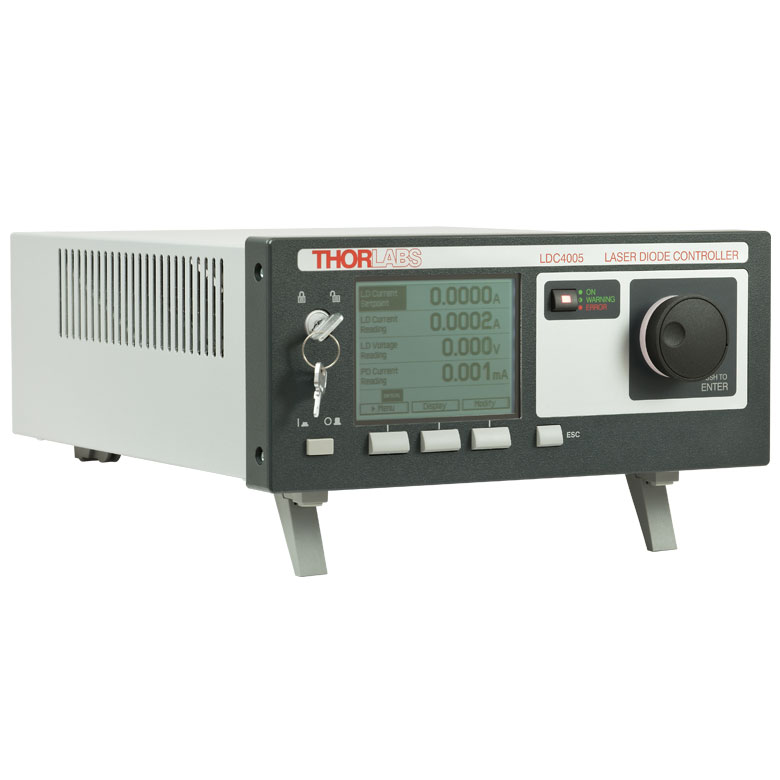
\includegraphics[width=0.30\textwidth,natwidth=69,natheight=87]{ldc4005.jpg}
\end{figure}
\item Miernik mocy firmy Thorlas firmy Thorlabs model PM100
\begin{figure}
%\hspace{4cm}  \vspace{1cm}
   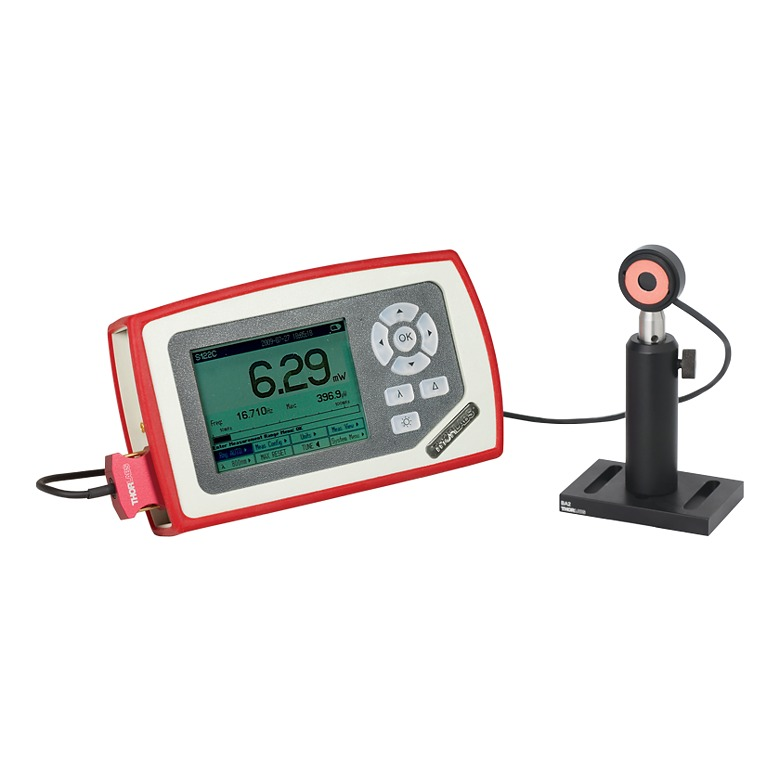
\includegraphics[width=0.30\textwidth,natwidth=69,natheight=87]{pm100.jpg}
\end{figure}
\end{itemize}
\end{frame}

\begin{frame}
\frametitle{Układ pomiarowy}
\begin{figure}
%\hspace{4cm}  \vspace{1cm}
   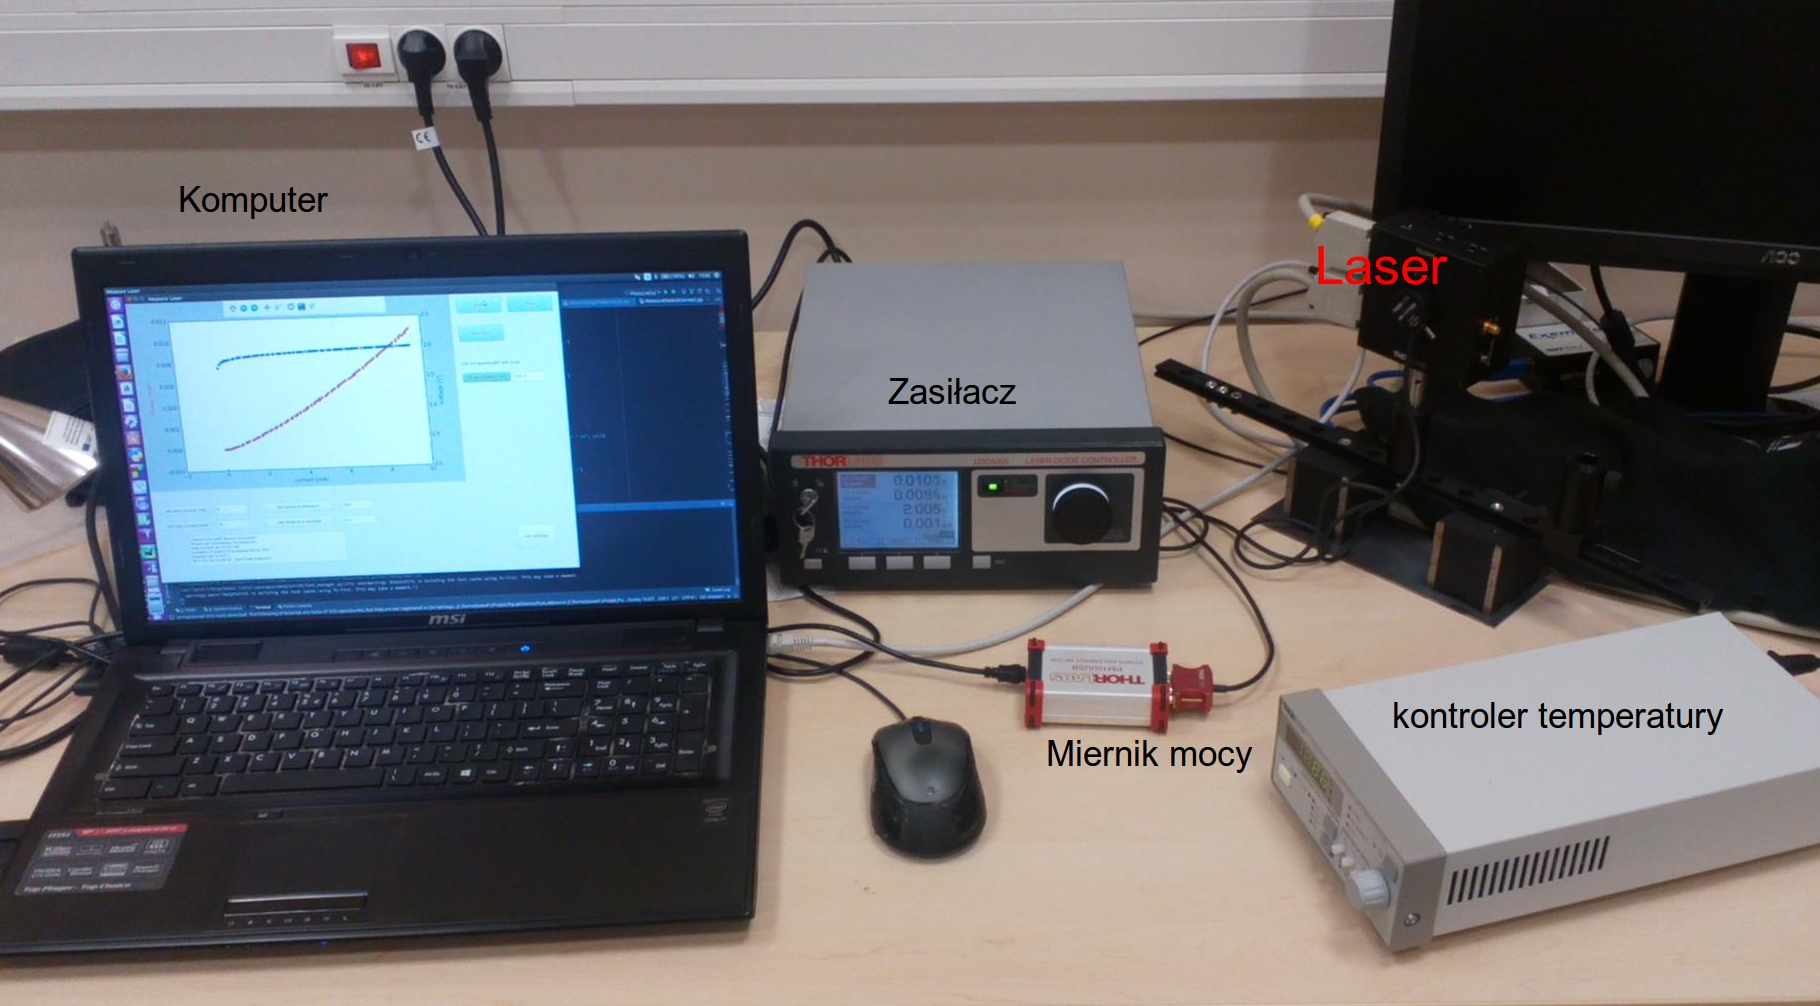
\includegraphics[width=0.85\textwidth,natwidth=69,natheight=87]{uklad.jpg}
\end{figure}
\end{frame}


\begin{frame}
\frametitle{Komunikacja z urządzenimi}
\begin{itemize}
\item SCPI (ang. Standard Commands for Programmable Instruments) --- język komend do urządzeń pomiarowych.
\item Wywołania systemowe (ang. System call)
\end{itemize}
SCPI + Wywołania systemowe = komunikacja z sprzętem laboratoryjnym
\end{frame}

\begin{frame}
\frametitle{SCPI --- Standard Commands for Programmable Instruments}
Standardowe polecenia programowanych urządzeń jest to standard komunikacji
\begin{itemize}
\item z urządzeniami pomiarowymi (oscyloskop, miernik mocy).
\item z urządzeniami laboratoryjnymi (zasiłacz)
\end{itemize} 
\end{frame}

\begin{frame}
\frametitle{SCPI --- przykłady}
\begin{itemize}
\item Komendy uniwersalne dla każdego urządzenia:
\begin{itemize}
\item $\mathtt{*rst}$ --- wyzerowanie urządzenia.
\item $\mathtt{*idn?}$ --- zapytanie o identyfikator.
\end{itemize}
\item Komendy specyficzny dla danego urządzenia:
\begin{itemize}
\item $\mathtt{SOURce:CURRent:LEVel:AMPLitude}$  $\mathtt{0.01}$
\end{itemize}
\end{itemize}
\end{frame}

\begin{frame}
\frametitle{Wywołania systemowe}
Interfejs pomiędzy programem użytkownika a jądrem Linux.
\begin{itemize}
\item $\mathtt{open}$.
\item $\mathtt{write}$.
\item $\mathtt{read}$.
\item $\mathtt{close}$.
\end{itemize}
\end{frame}

\begin{frame}
\frametitle{Przykładowy program}
\lstinputlisting[language=Python, firstline=0, lastline=20]{deviceio.py}
\end{frame}

\begin{frame}
\frametitle{Skrypt}
\begin{itemize}
\item $\mathtt{sudo}$ $\mathtt{su}$
\item $\mathtt{python3}$ measure.py -nr 150 -sc 0 -ec 25 -fn data.txt

\end{itemize}
\end{frame}

\begin{frame}
\frametitle{Program okienkowy do pomiarów}
\begin{figure}
%\hspace{4cm}  \vspace{1cm}
   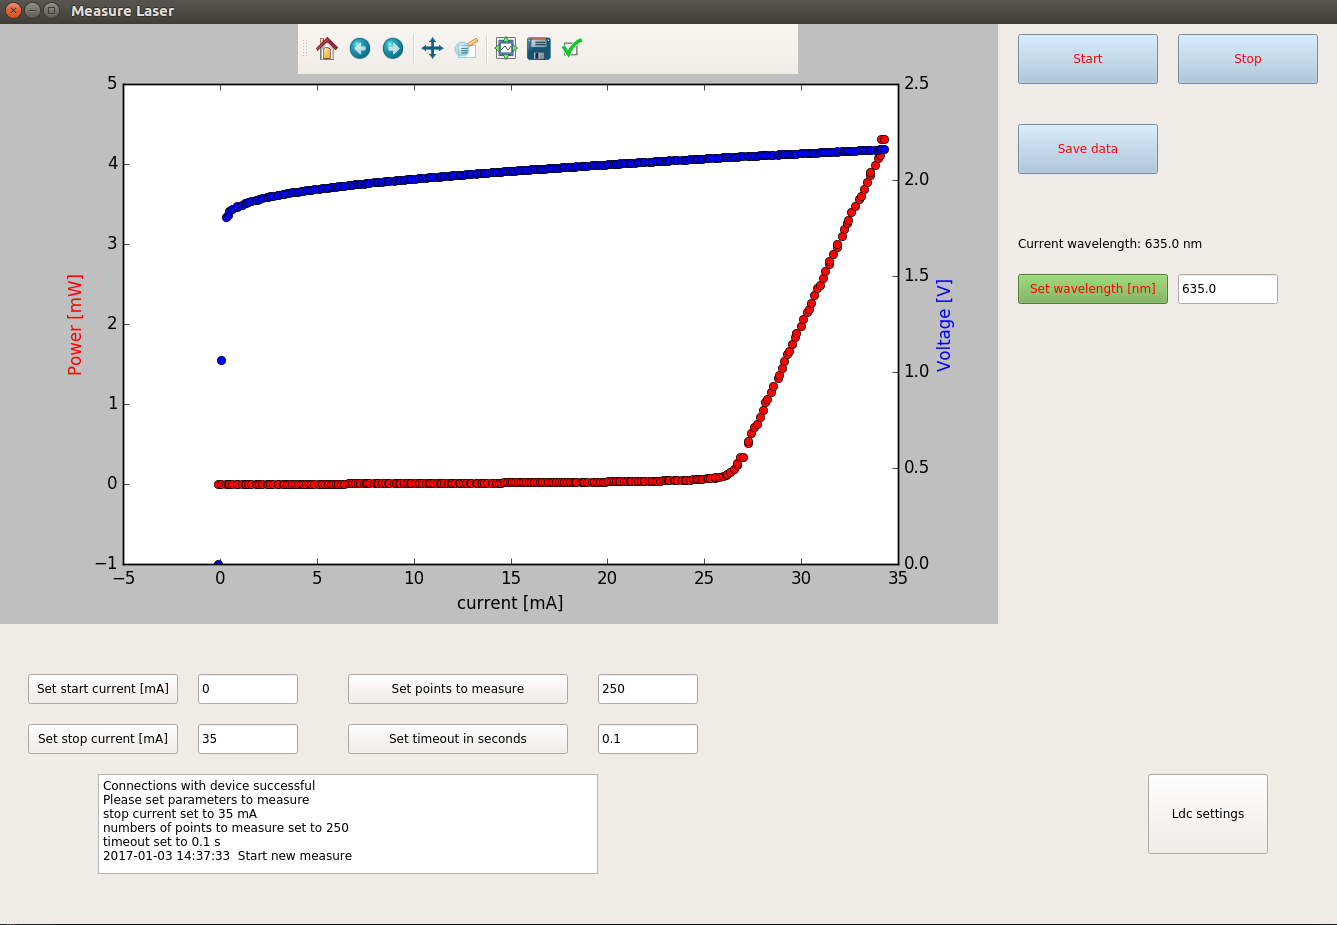
\includegraphics[width=0.85\textwidth,natwidth=69,natheight=87]{gui.png}
\end{figure}
\end{frame}

\begin{frame}
\begin{Huge}
\begin{center}
Eksperyment
\end{center}
\end{Huge}
\end{frame}

\begin{frame}
\frametitle{Teoria --- prąd progowy}
Prąd progowy (z ang. \textit{threshold current}) określa wartość prądu przy którym zaczyna zachodzić akcja laserowa czyli rośnie gwałtownie natężenie promieniowania i maleje szerokość linii emisyjnej.
\begin{figure}
%\hspace{4cm}  \vspace{1cm}
   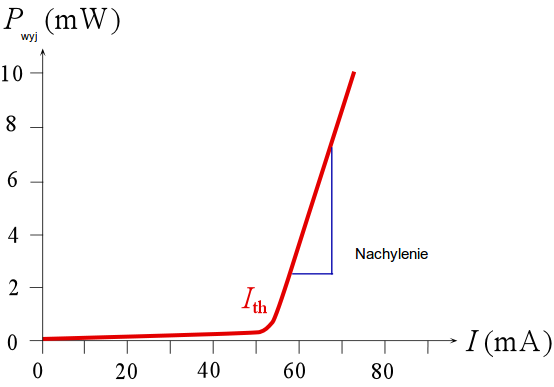
\includegraphics[width=0.65\textwidth,natwidth=69,natheight=87]{slope.png}
\end{figure}
\end{frame}

\begin{frame}
\frametitle{Prąd progowy --- wykres}
\begin{figure}
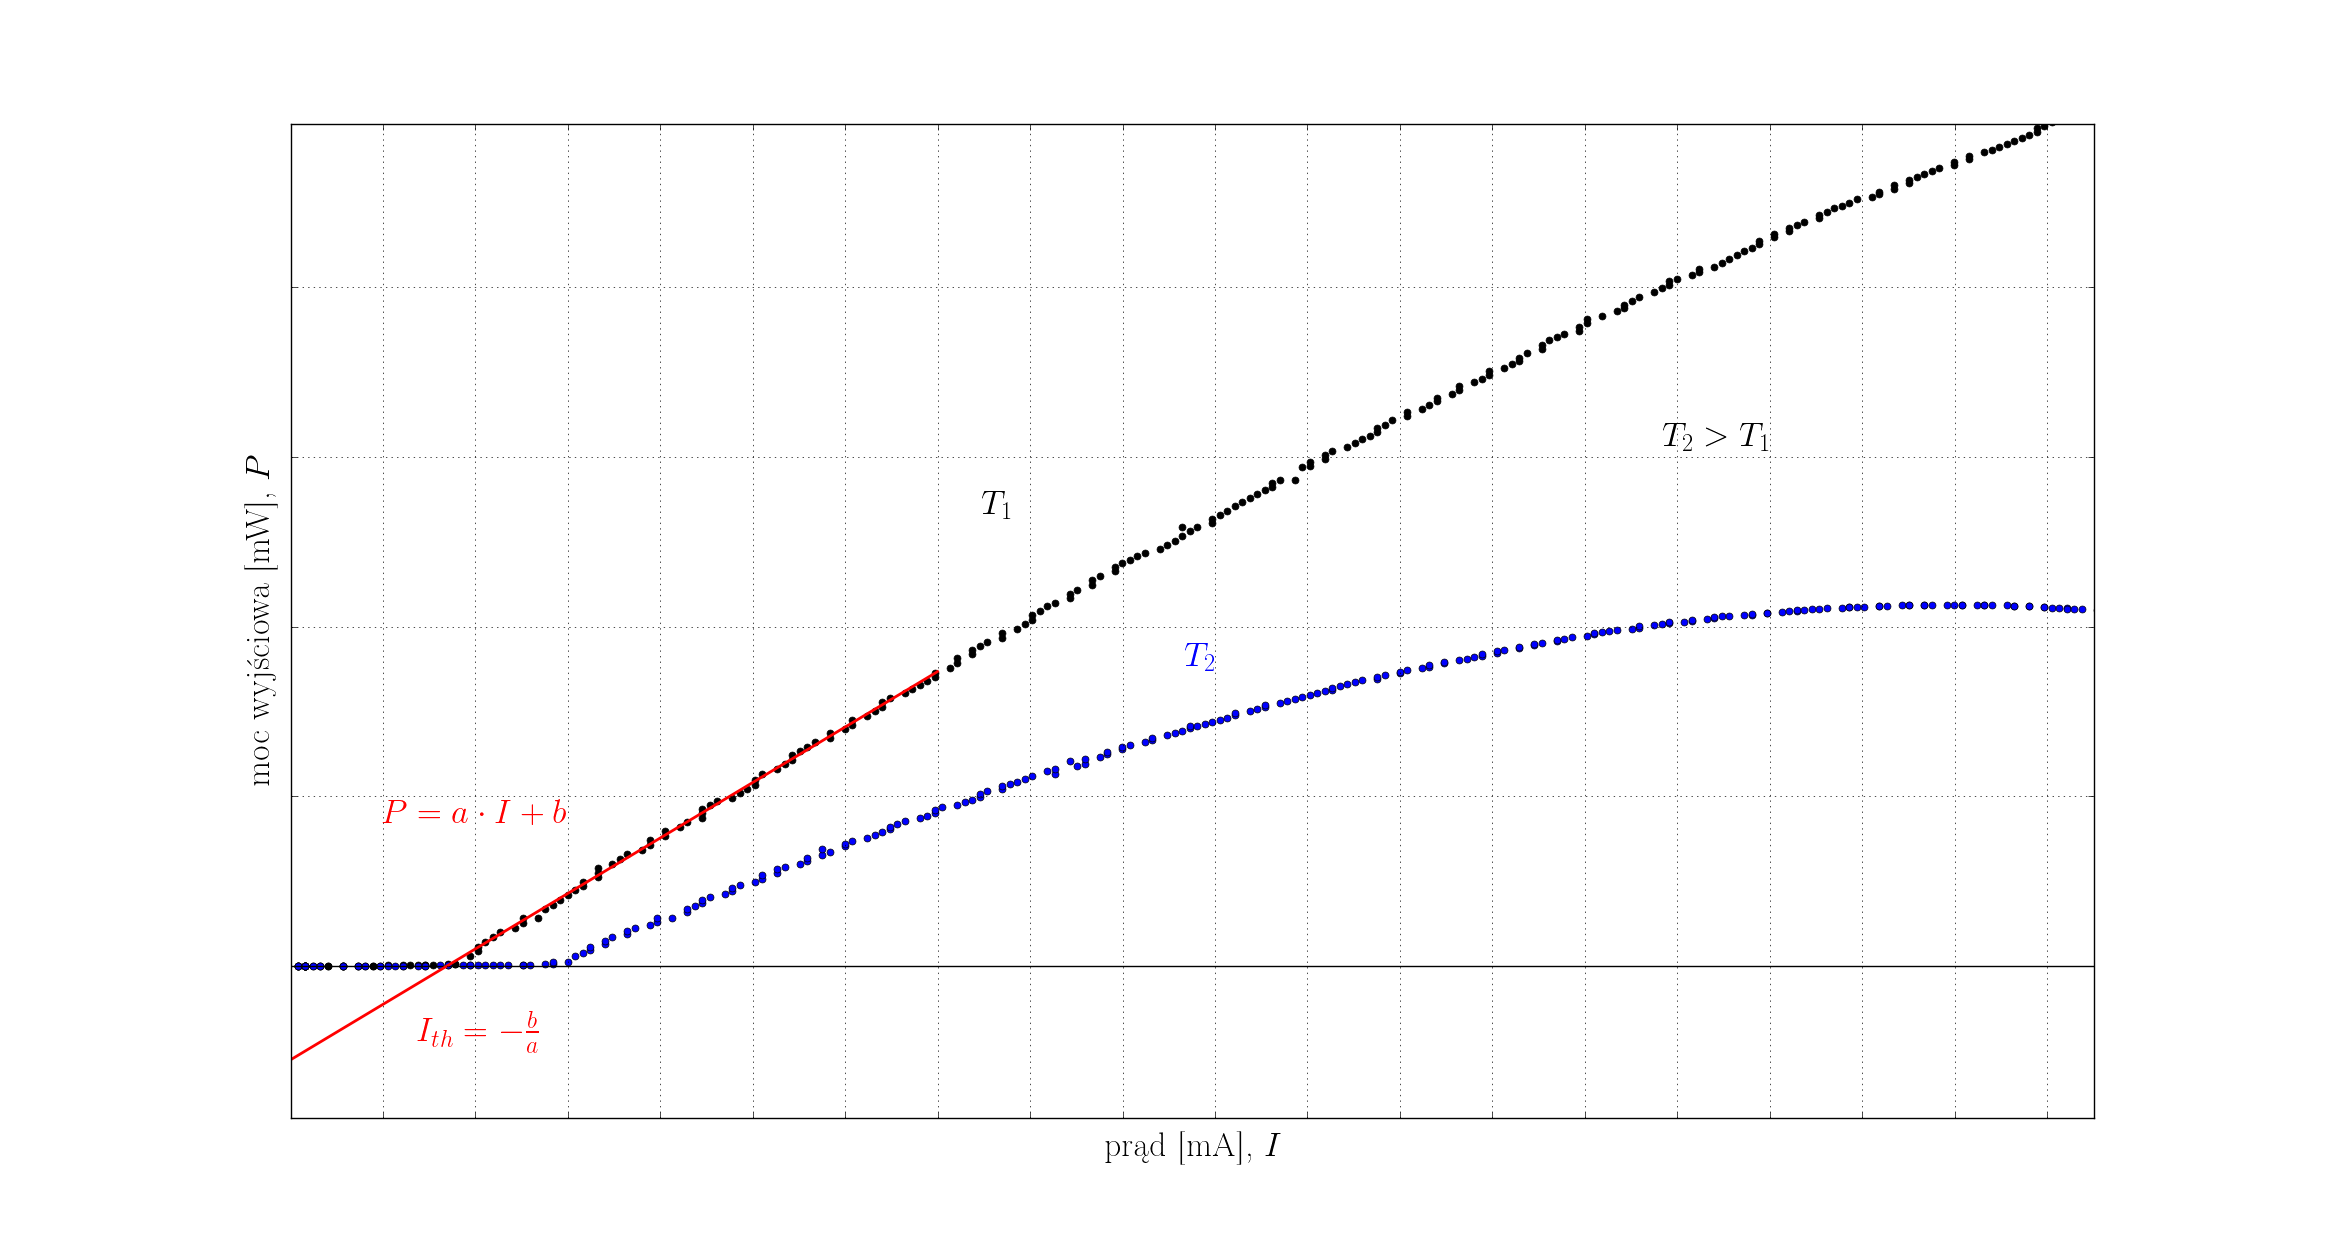
\includegraphics[scale=0.20]{plot_theory.png}
\end{figure}
\end{frame}

\begin{frame}
\frametitle{Prąd progowy}
\center
\begin{equation*}
I_{\mathtt{th}} = -\frac{b}{a}
\end{equation*}
\begin{equation*}
\Delta I_{th} = \left\lvert \frac{\partial I_{th}}{\partial a} \right\rvert \cdot \Delta a + \left\lvert \frac{\partial I_{th}}{\partial b} \right\rvert \cdot \Delta b
\end{equation*}
\begin{equation*}
\Delta I_{th} = \left\lvert -\frac{b}{a^2} \right\rvert \cdot \Delta a + \left\lvert -\frac{1}{a} \right\rvert \cdot \Delta b 
\end{equation*}

\end{frame}

\begin{frame}
\frametitle{Prąd progowy zależność od temperatury}

\begin{equation*}
I_{th} = I_0 \exp \left( \frac{T}{T_0} \right)
\end{equation*}
\begin{equation*}
\ln (I_{th}) =  \ln \frac{T}{T_0}  + \ln(I_{0})
\end{equation*}
\begin{equation*}
y = a \cdot T + b
\end{equation*}

\begin{equation*}
y = \ln(I_{th})
\end{equation*}
\begin{equation*}
a = \frac{1}{T_0} \Rightarrow T_0 = \frac{1}{a}
\end{equation*}
\begin{equation*}
b = \ln(I_0) \Rightarrow I_0 = e^b
\end{equation*}
\end{frame}

\begin{frame}
\frametitle{Prąd progowy   w zależności od temperatury--- wyznaczenie błędów pomiarowych}
\center
\begin{equation*}
T_0 = \frac{1}{a}
\end{equation*}
\begin{equation*}
I_0 = e^b
\end{equation*}


\begin{equation*}
\Delta T_0 = \left\lvert \frac{\partial T_{0}}{\partial a} \right\rvert \cdot \Delta a = \left\lvert -\frac{1}{a^2} \right\rvert \cdot \Delta a
\end{equation*}
\begin{equation*}
\Delta I_0 = \left\lvert \frac{\partial I_{0}}{\partial b} \right\rvert \cdot \Delta b = | b \mathtt{e}^b | \cdot \Delta b
\end{equation*}

\end{frame}

\begin{frame}
\frametitle{Sprawność}
\begin{itemize}
\item Moc wyjściowa  ---  mierzymy na mierniku mocy.
\item Moc wejściowa --- iloczyn prądu $I$ i napięcia $U$.
\begin{equation*}
P_{in} = I \cdot U
\end{equation*}
\end{itemize}
\end{frame}

\begin{frame}
\center
\begin{figure}
%\hspace{4cm}  \vspace{1cm}
   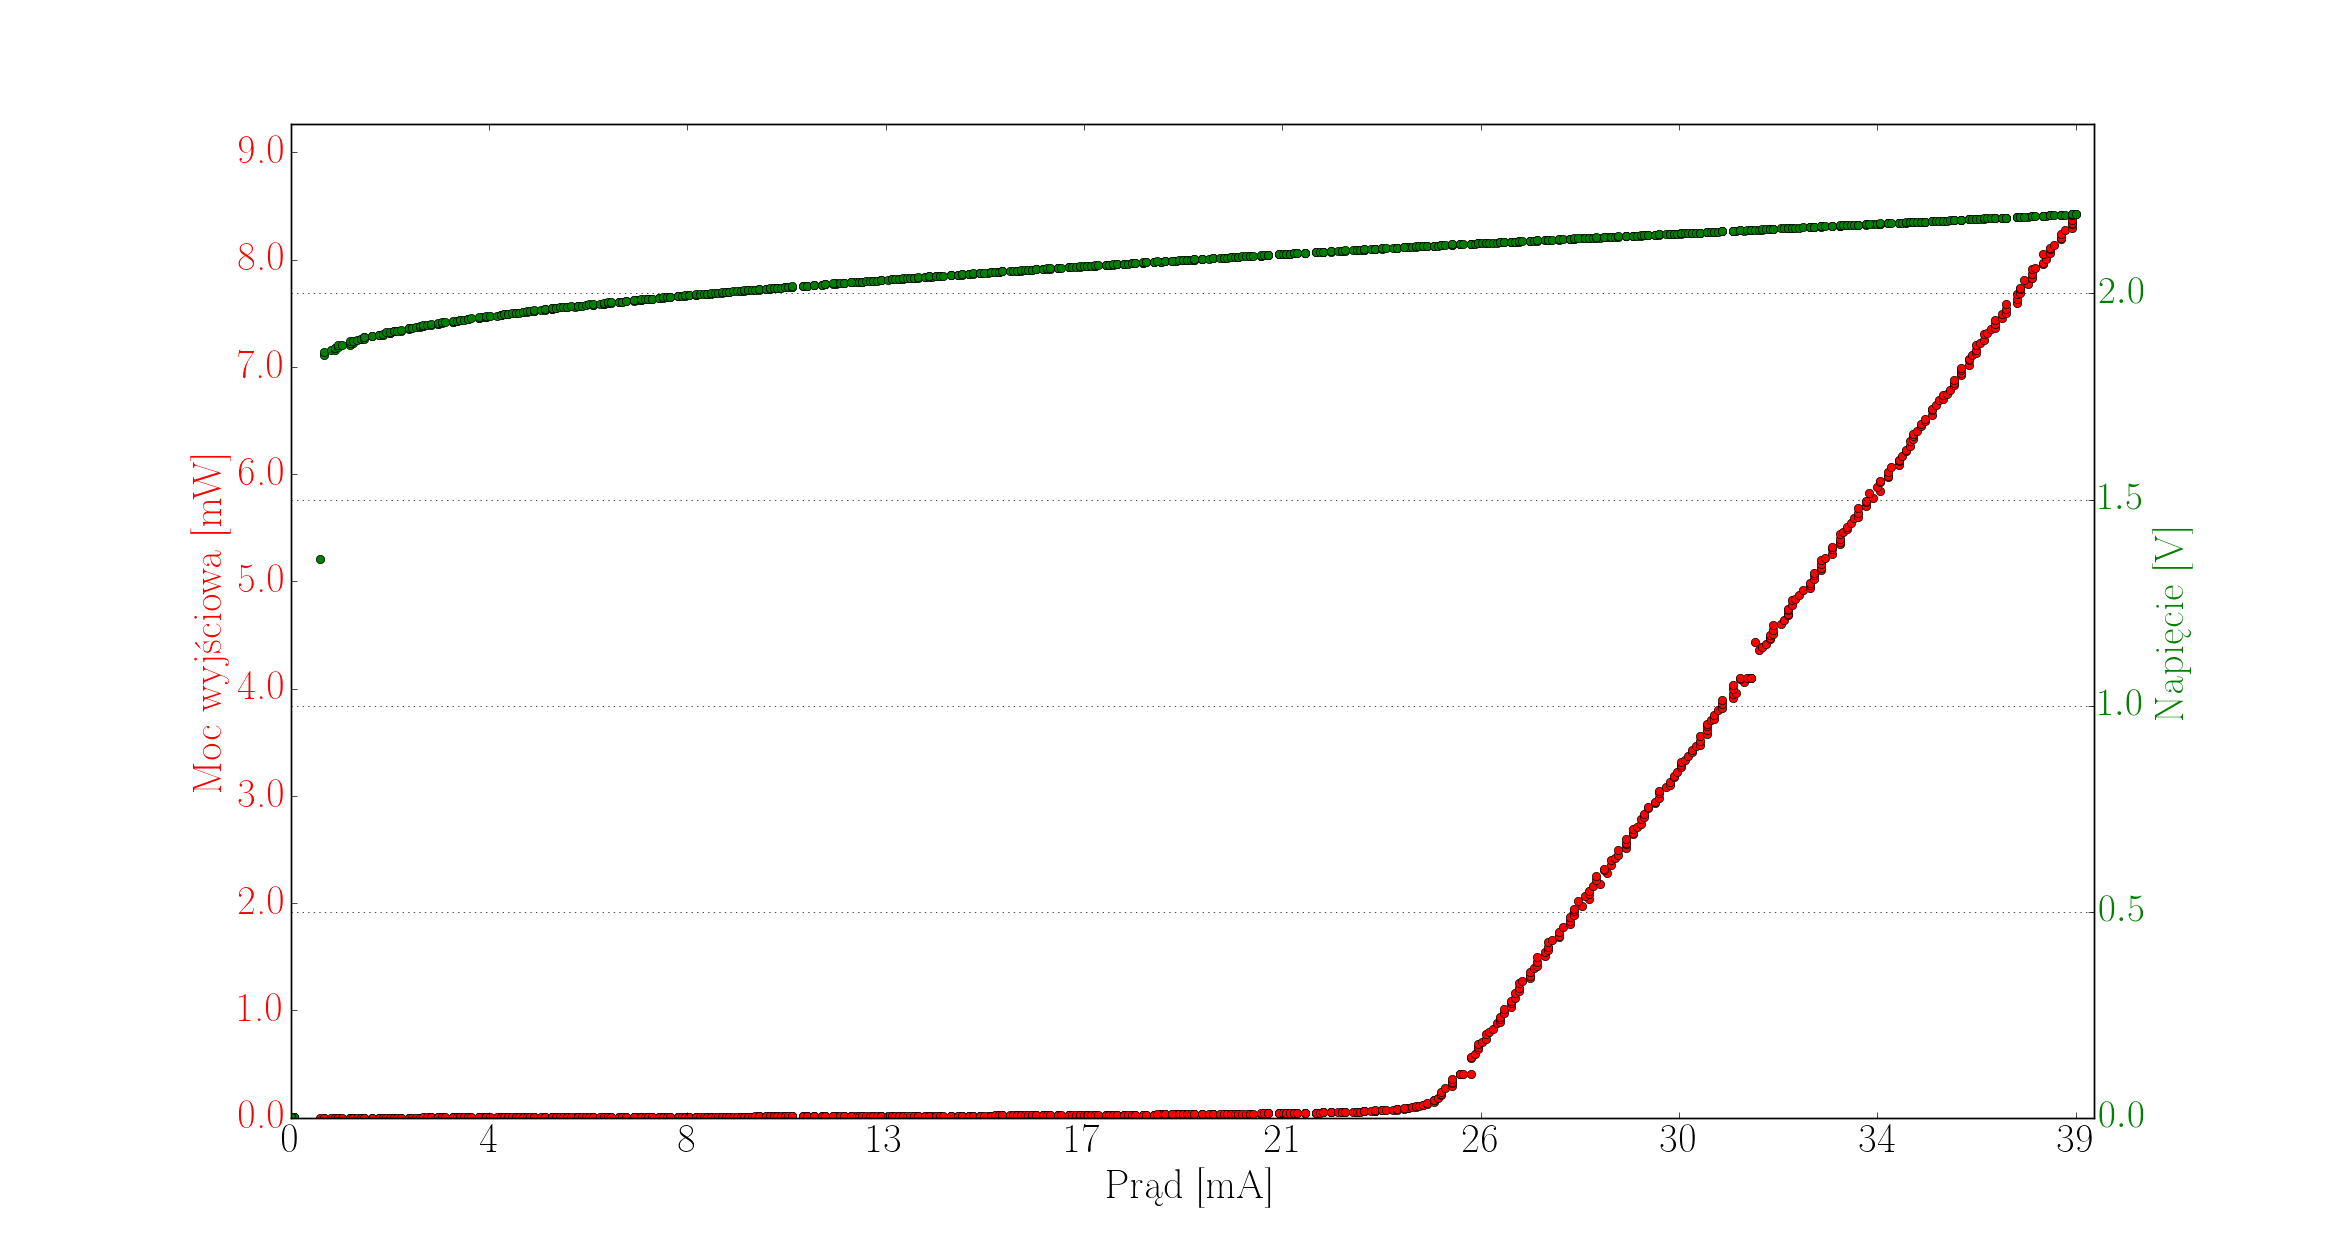
\includegraphics[width=1.10\textwidth,natwidth=69,natheight=87]{635/plot_ivl_25.png}
\end{figure}

\end{frame}

\begin{frame}
\center
\begin{figure}
%\hspace{4cm}  \vspace{1cm}
   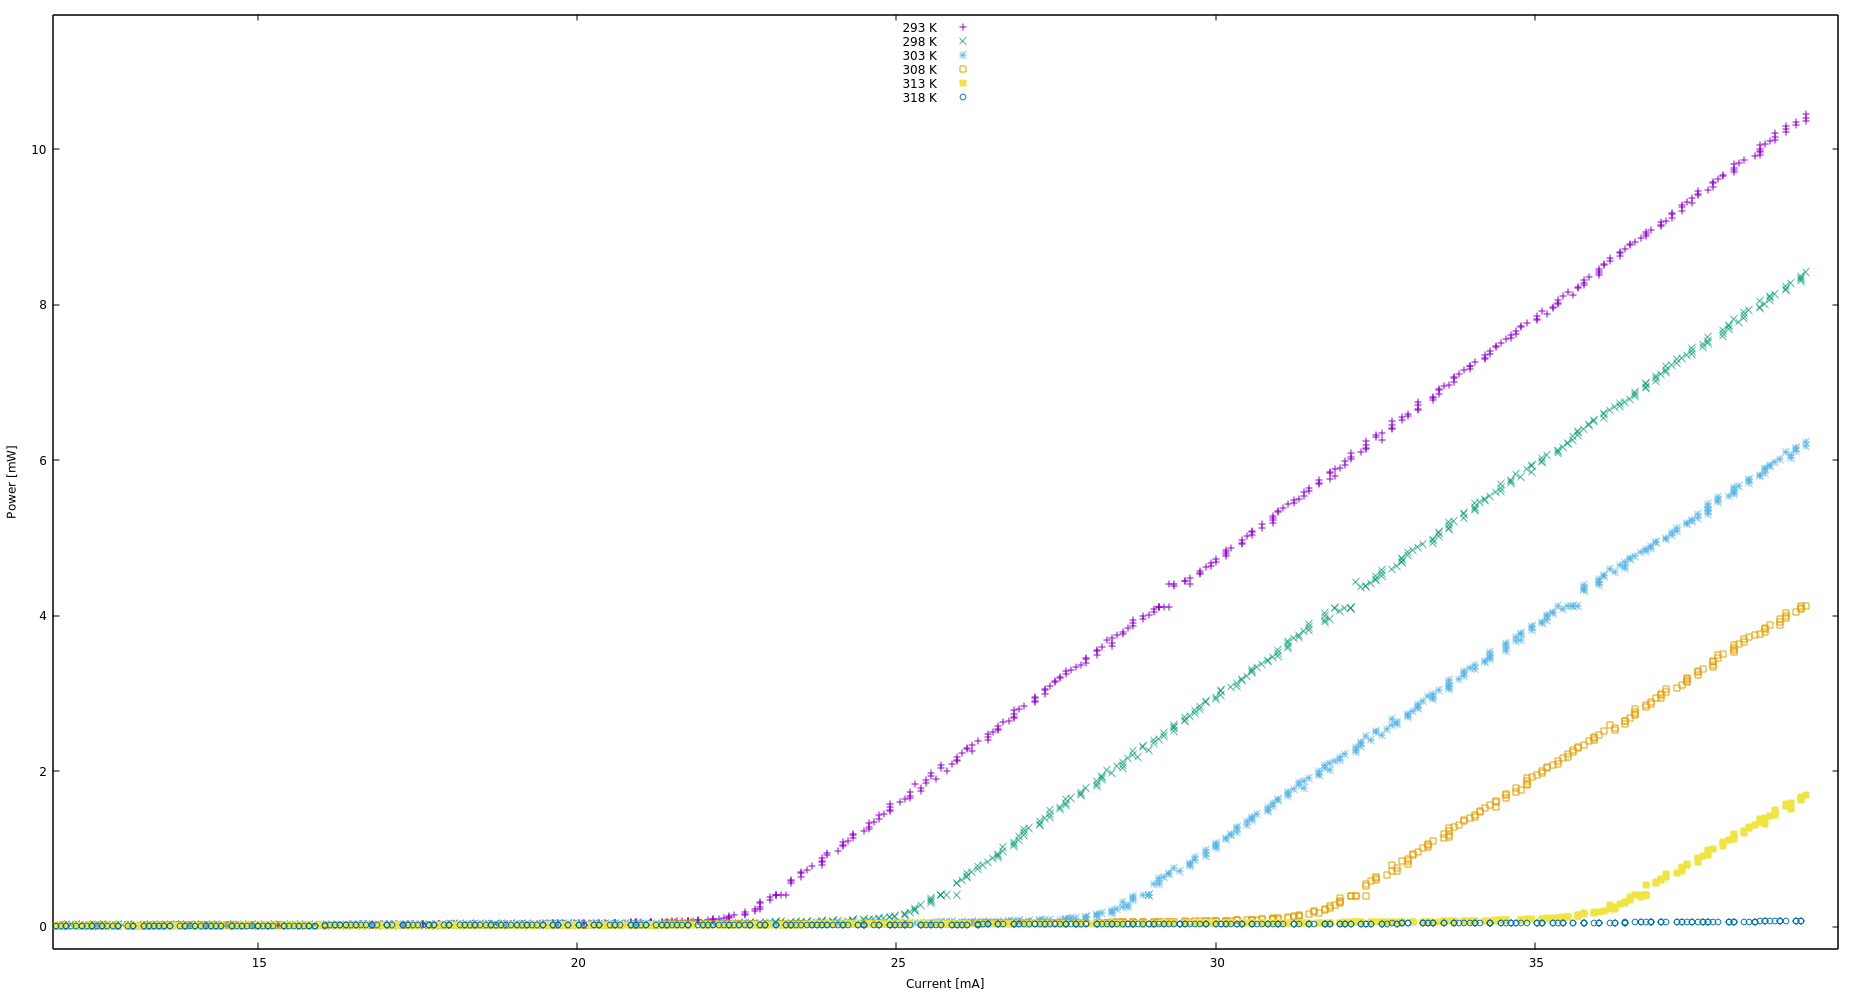
\includegraphics[width=1.0\textwidth,natwidth=69,natheight=87]{635/plot_all.png}
\end{figure}
\end{frame}



\begin{frame}
\frametitle{Laser 635\,nm w temperaturze 293\,K}
\center
\begin{figure}
%\hspace{4cm}  \vspace{1cm}
   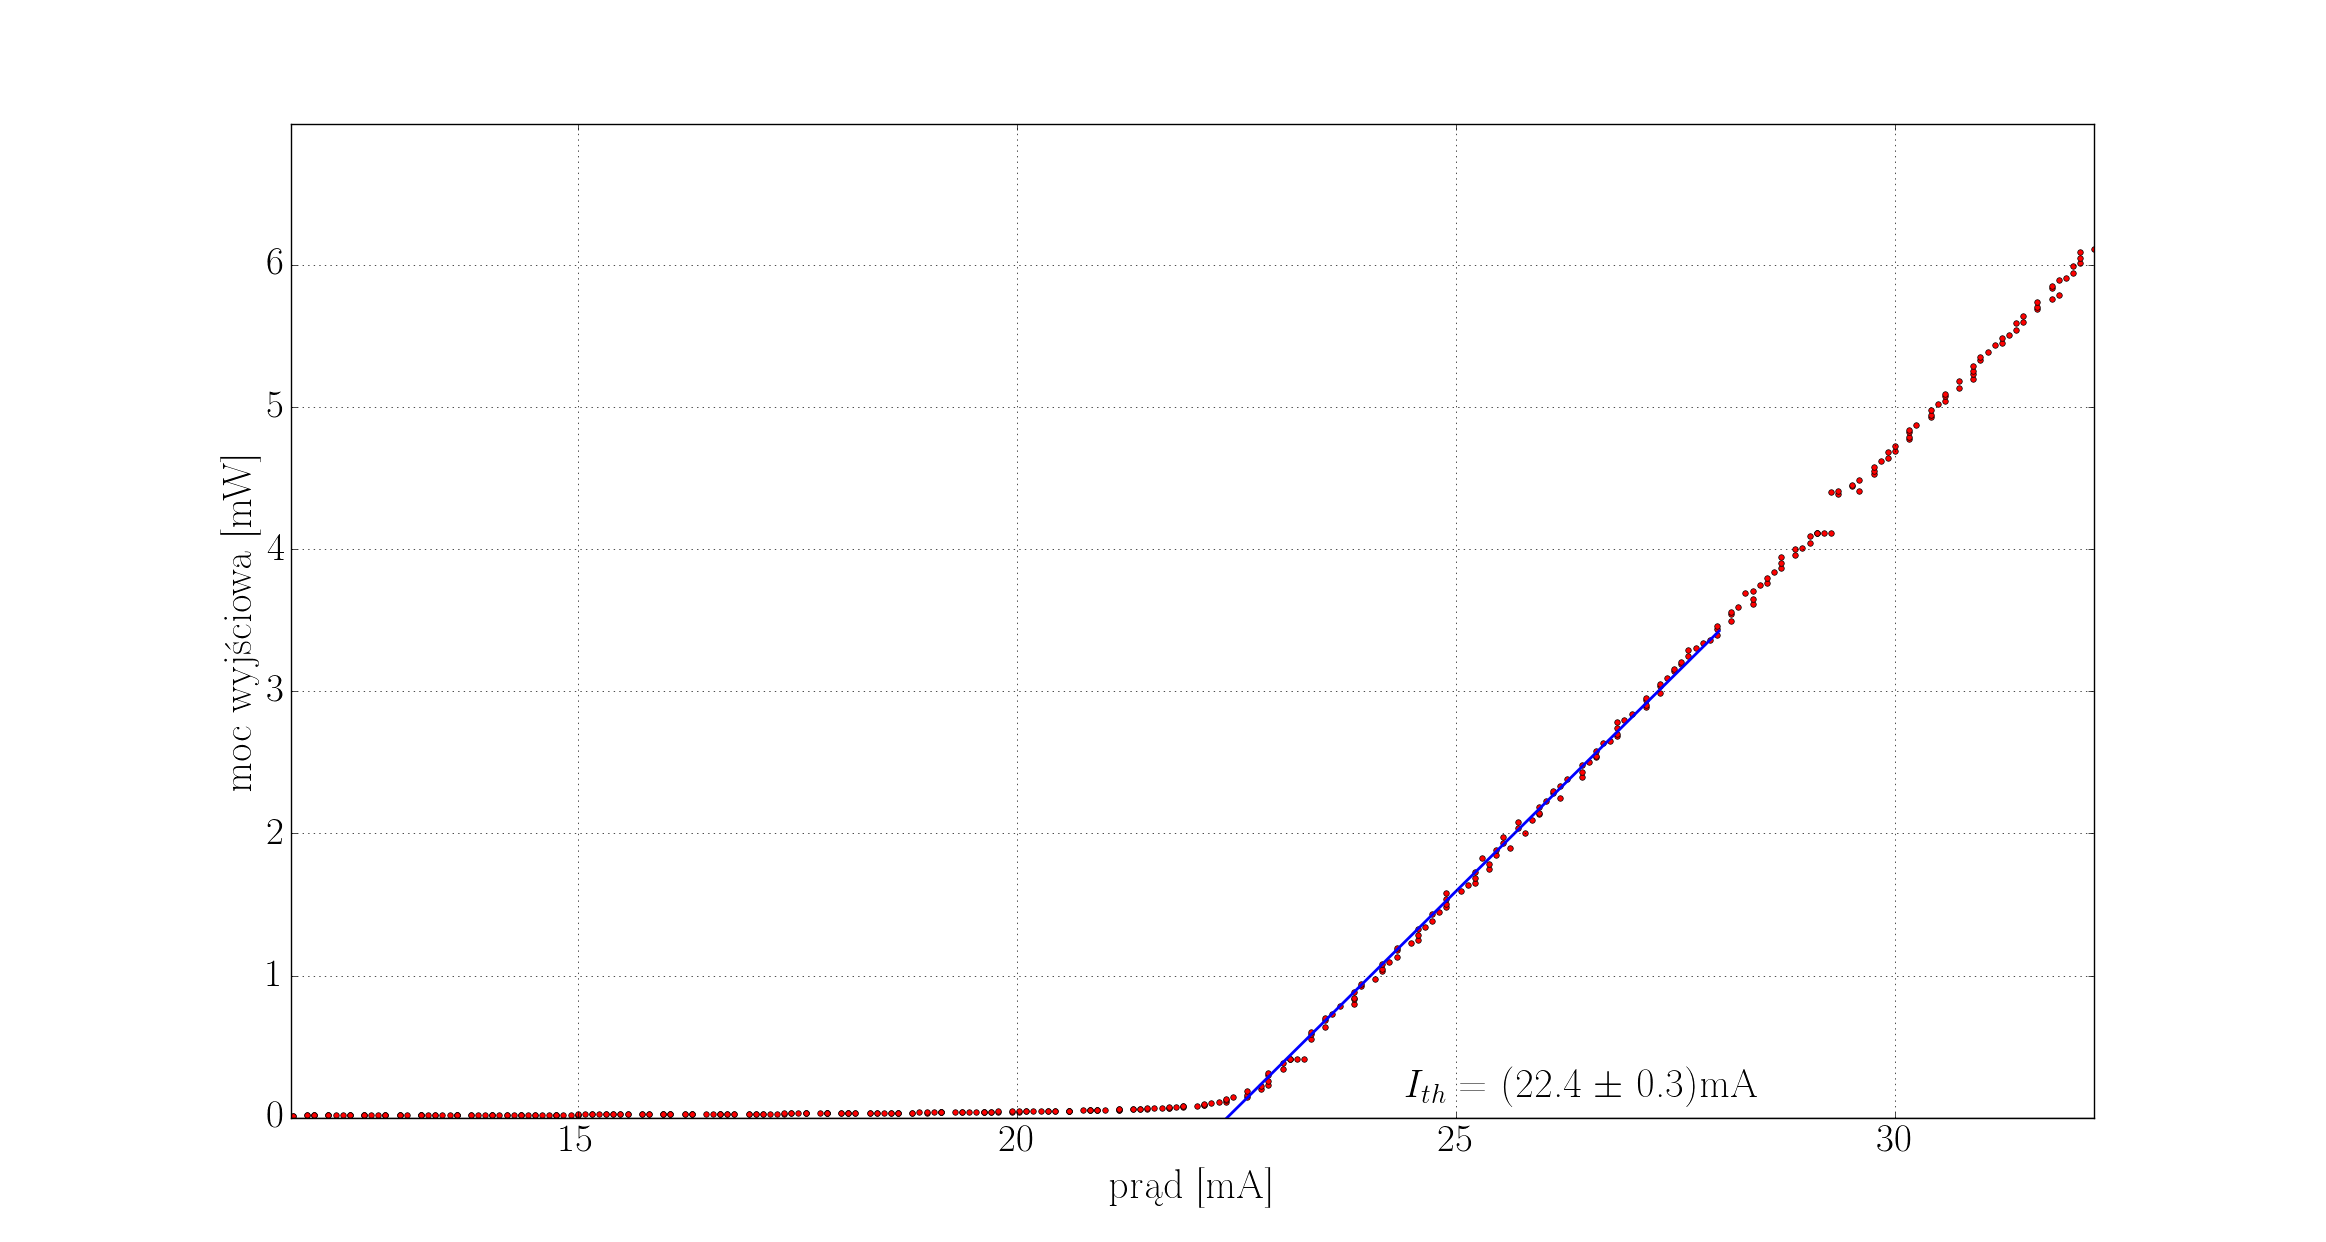
\includegraphics[width=1.10\textwidth,natwidth=69,natheight=87]{635/plot_i_th_20.png}
\end{figure}
\end{frame}

\begin{frame}
\frametitle{Laser 980\,nm w temperaturze 308\,K}
\center
\begin{figure}
%\hspace{4cm}  \vspace{1cm}
   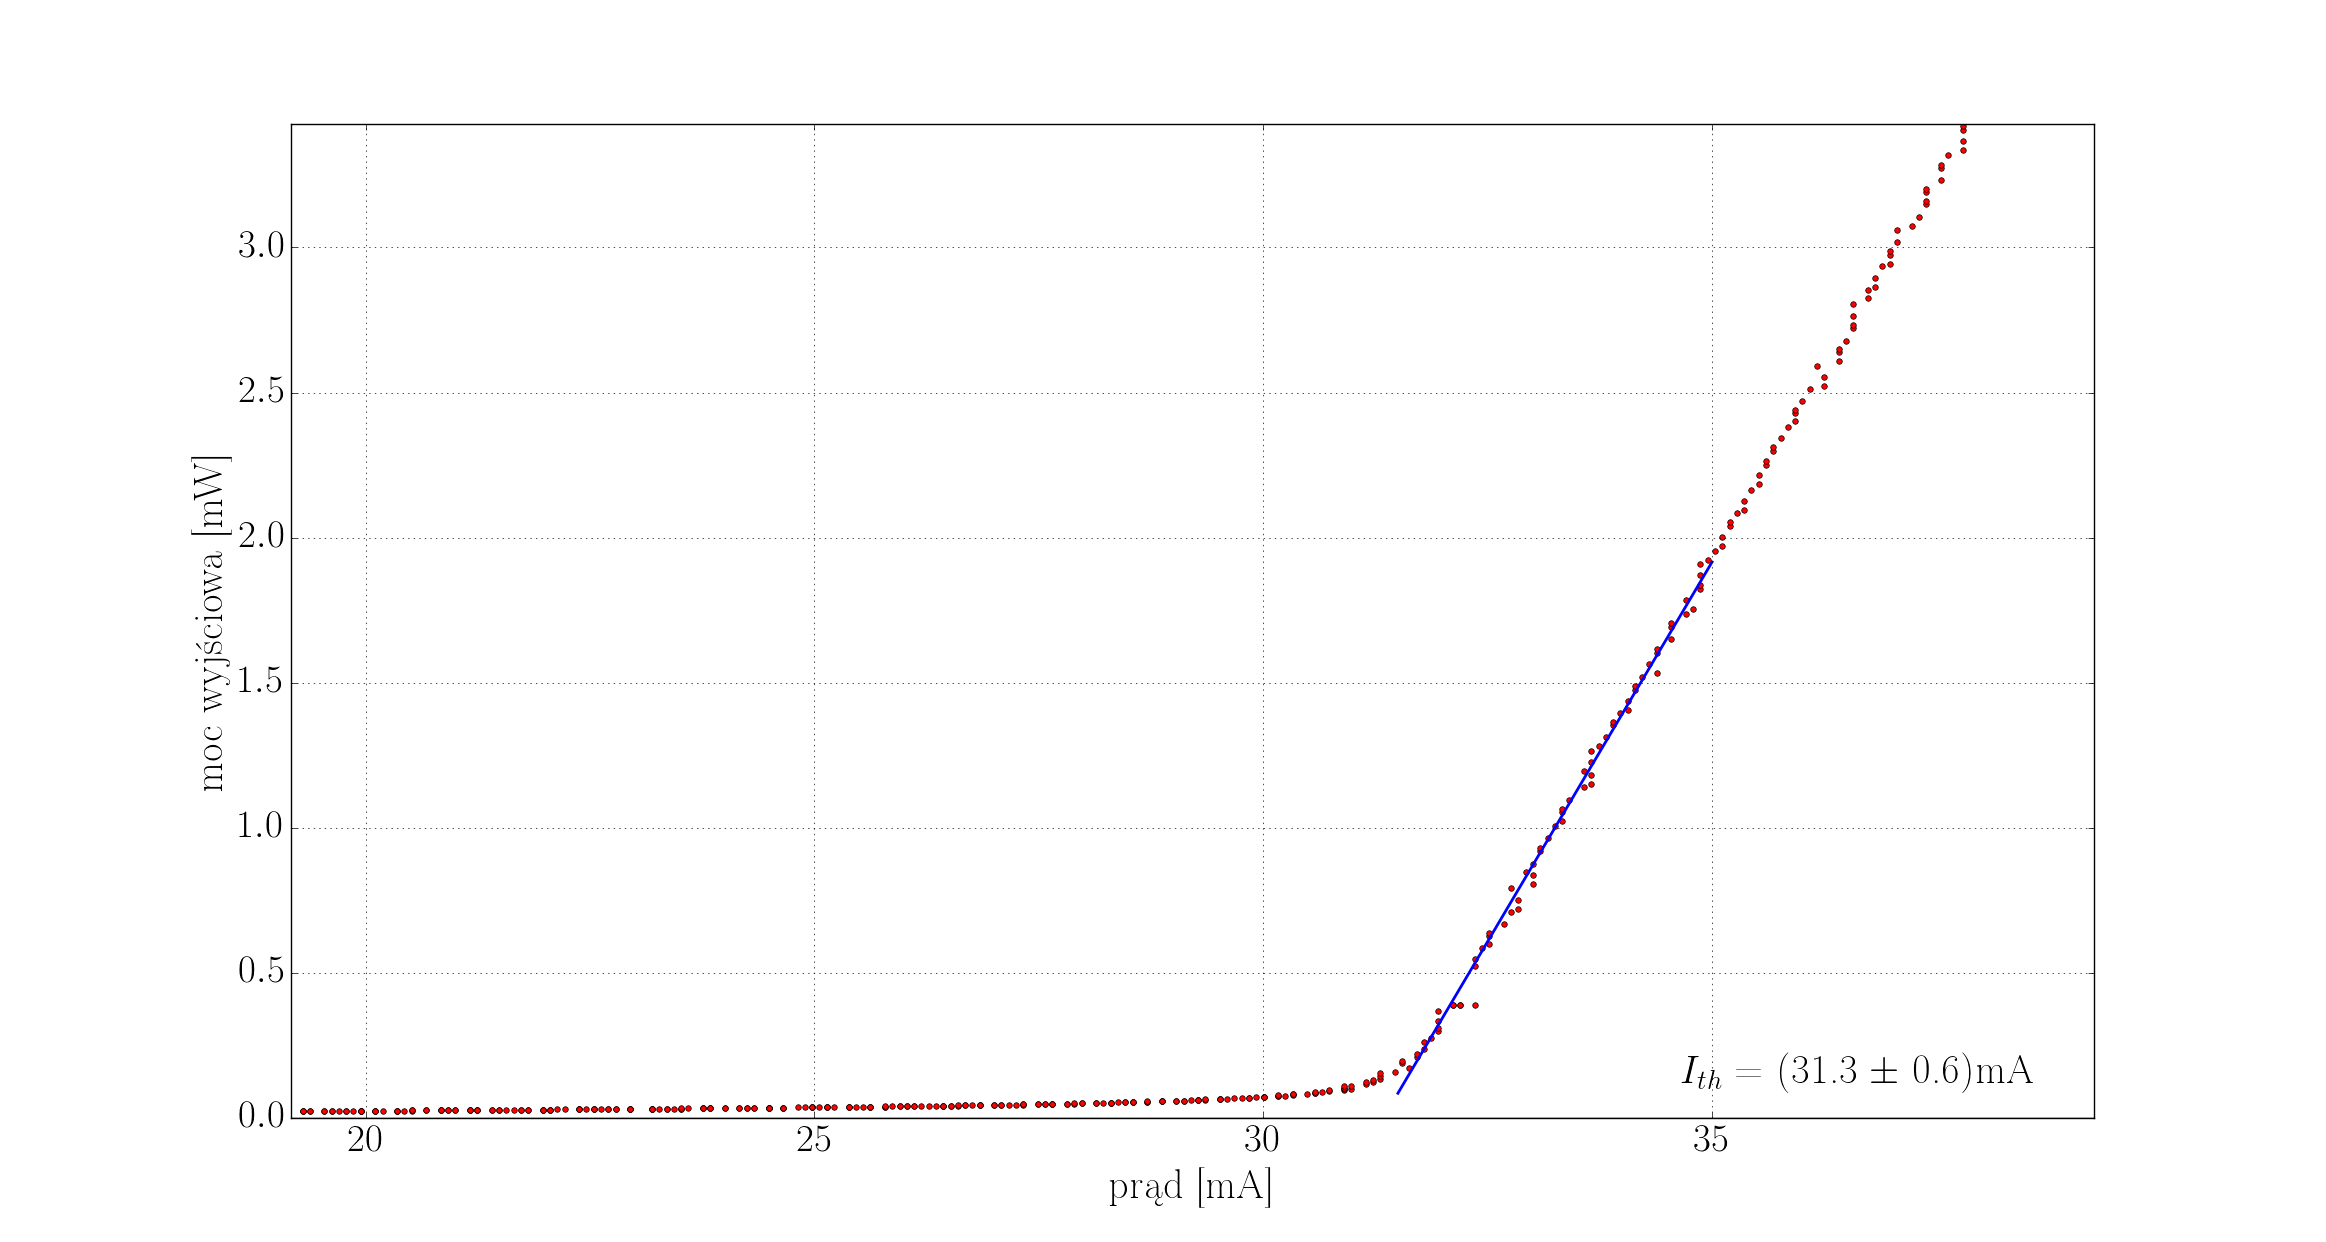
\includegraphics[width=1.10\textwidth,natwidth=69,natheight=87]{635/plot_i_th_35.png}
\end{figure}
\end{frame}


\begin{frame}
\frametitle{Wykres liniowy prądu progowego od temperatury}
\center
\begin{figure}
%\hspace{4cm}  \vspace{1cm}
   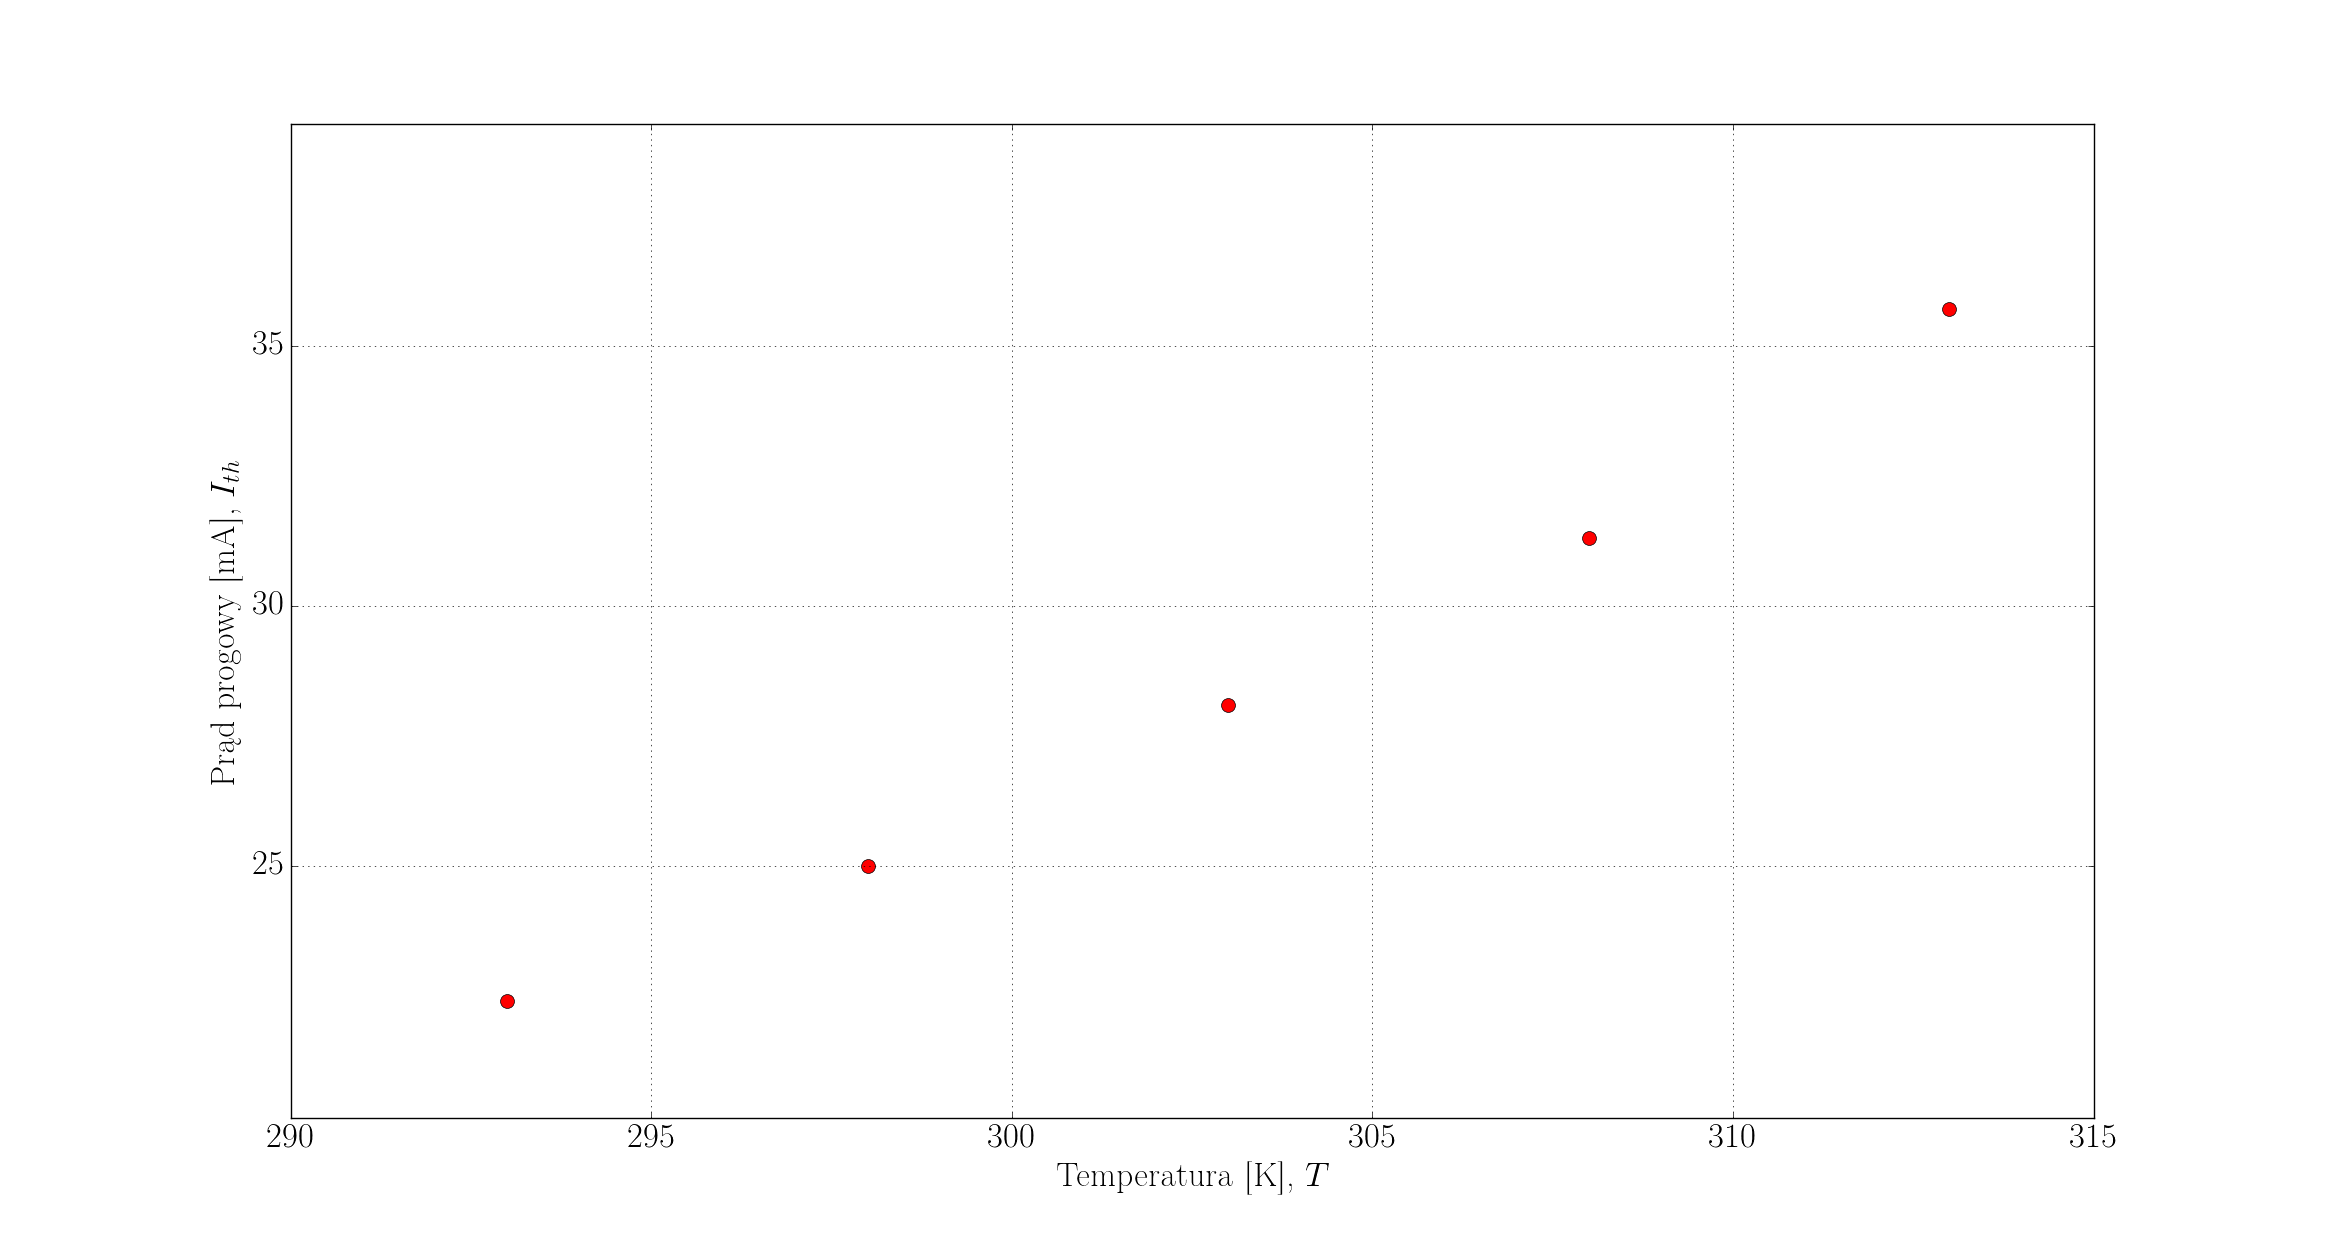
\includegraphics[width=1.10\textwidth,natwidth=69,natheight=87]{635/plot_lin_i_th.png}
\end{figure}
\end{frame}

\begin{frame}
\frametitle{Wykres logarytmu z prądu progowego od temperatury}
\center
\begin{figure}
%\hspace{4cm}  \vspace{1cm}
   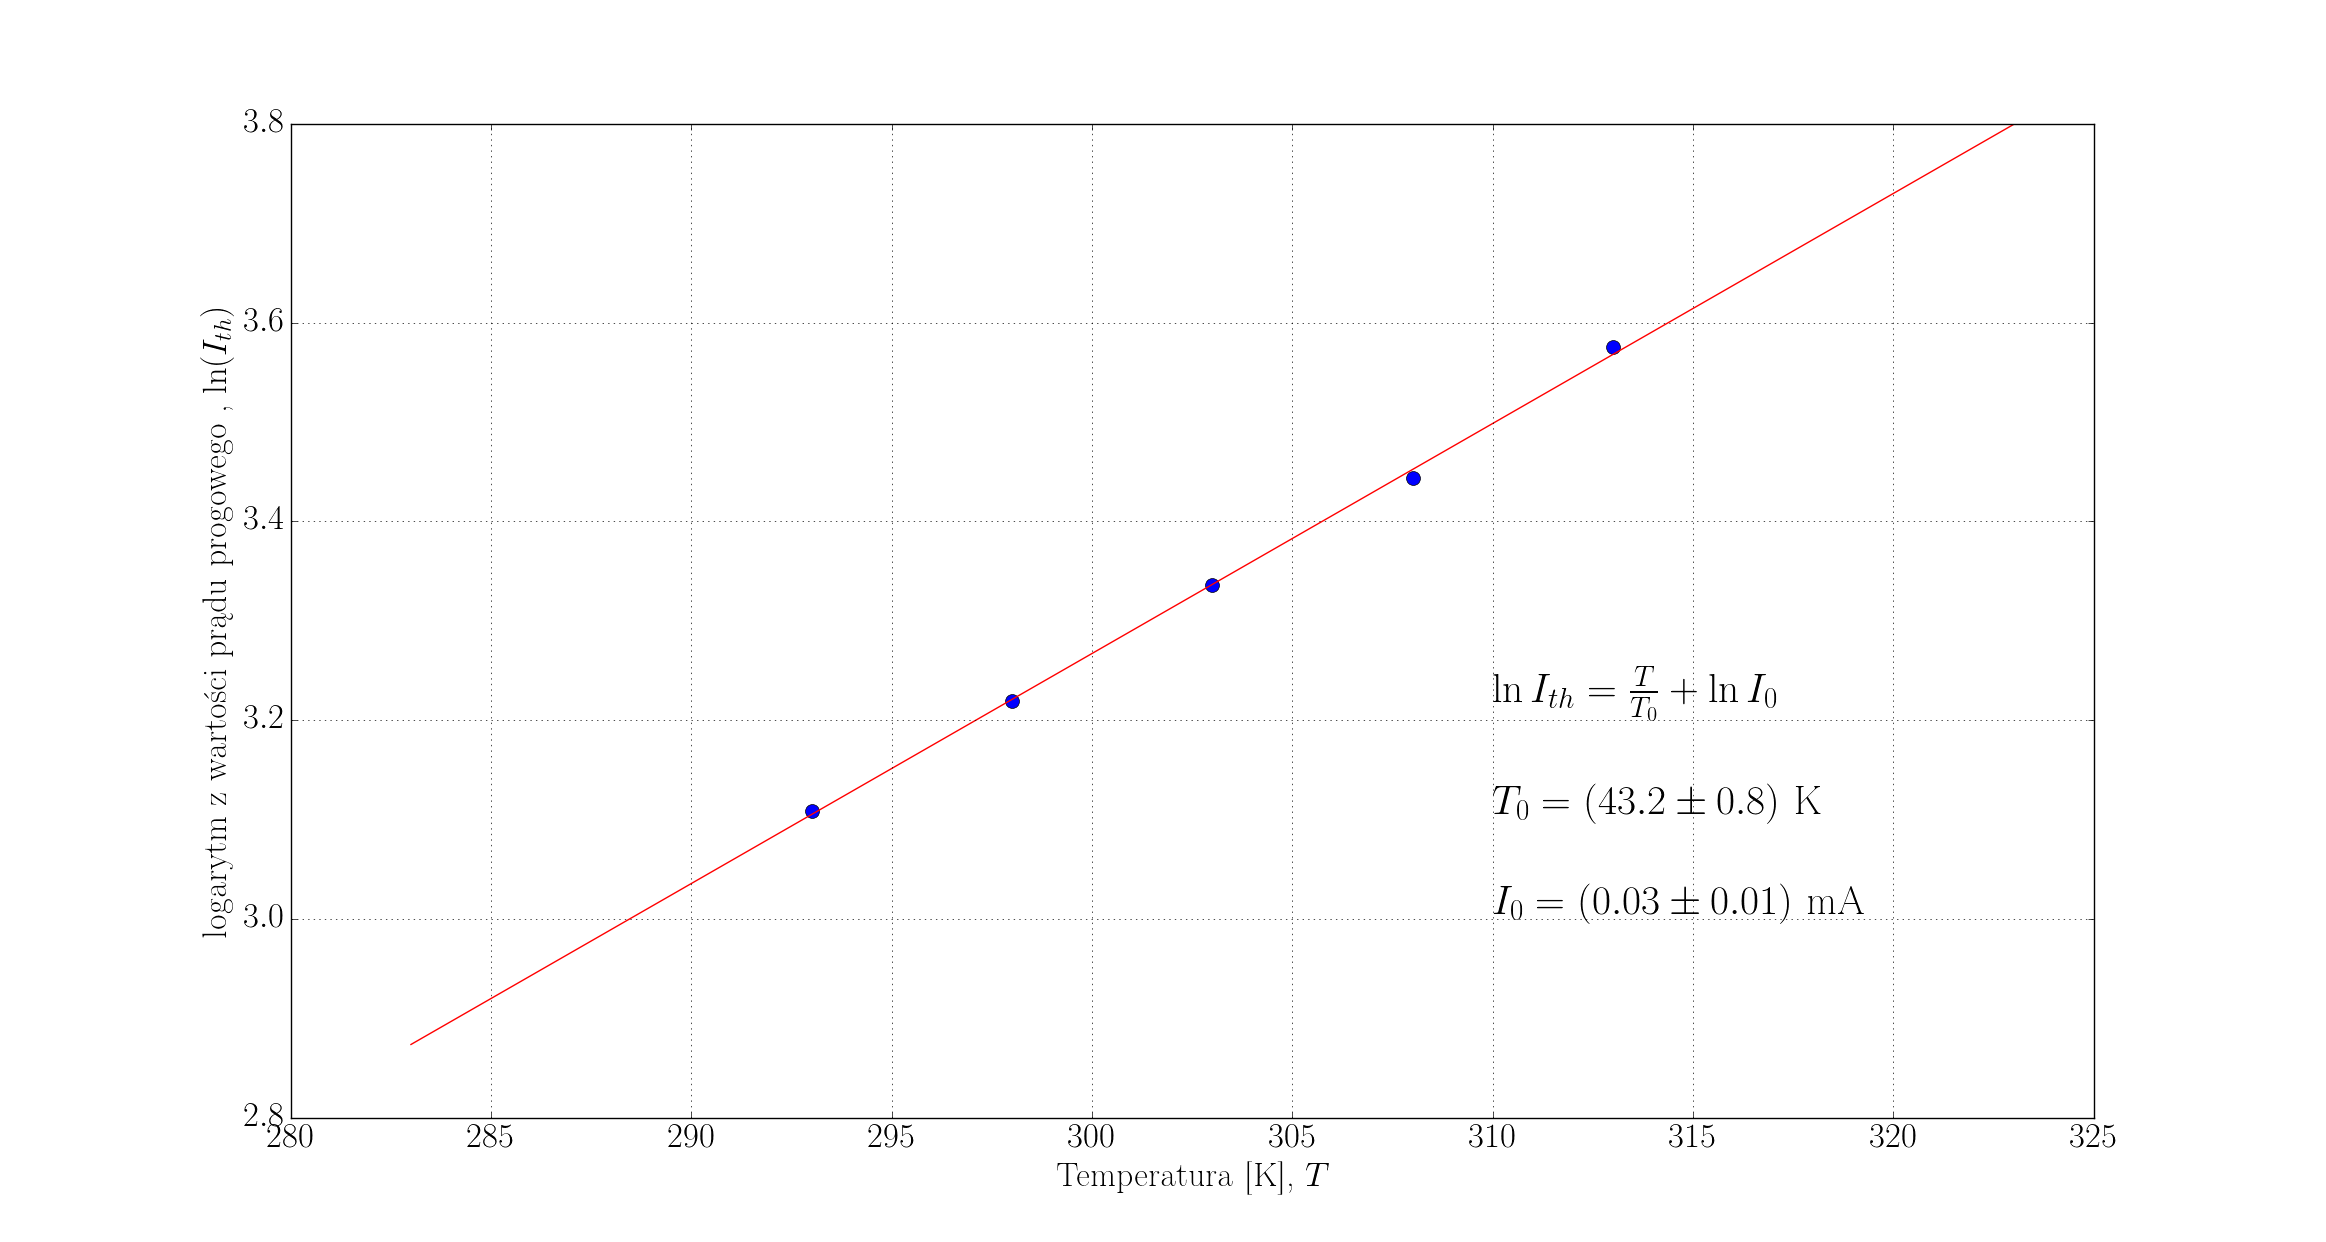
\includegraphics[width=1.10\textwidth,natwidth=69,natheight=87]{635/fit_i_0.png}
\end{figure}
\end{frame}

\begin{frame}
\frametitle{Laser krawędziowy 635\,nm --- wyznaczone parametry}
\begin{itemize}
\item $T_0 = (43.2 \pm 0.8)$\,K
\item $I_0 = (0.03 \pm 0.01)$\,mA
\end{itemize}
\begin{equation*}
I_{th} = 0.03 \cdot \exp \left( \frac{T}{43.2} \right)
\end{equation*}
\end{frame}

\begin{frame}
\frametitle{Laser krawędziowy 635\,nm --- wykres}
\center
\begin{figure}
%\hspace{4cm}  \vspace{1cm}
   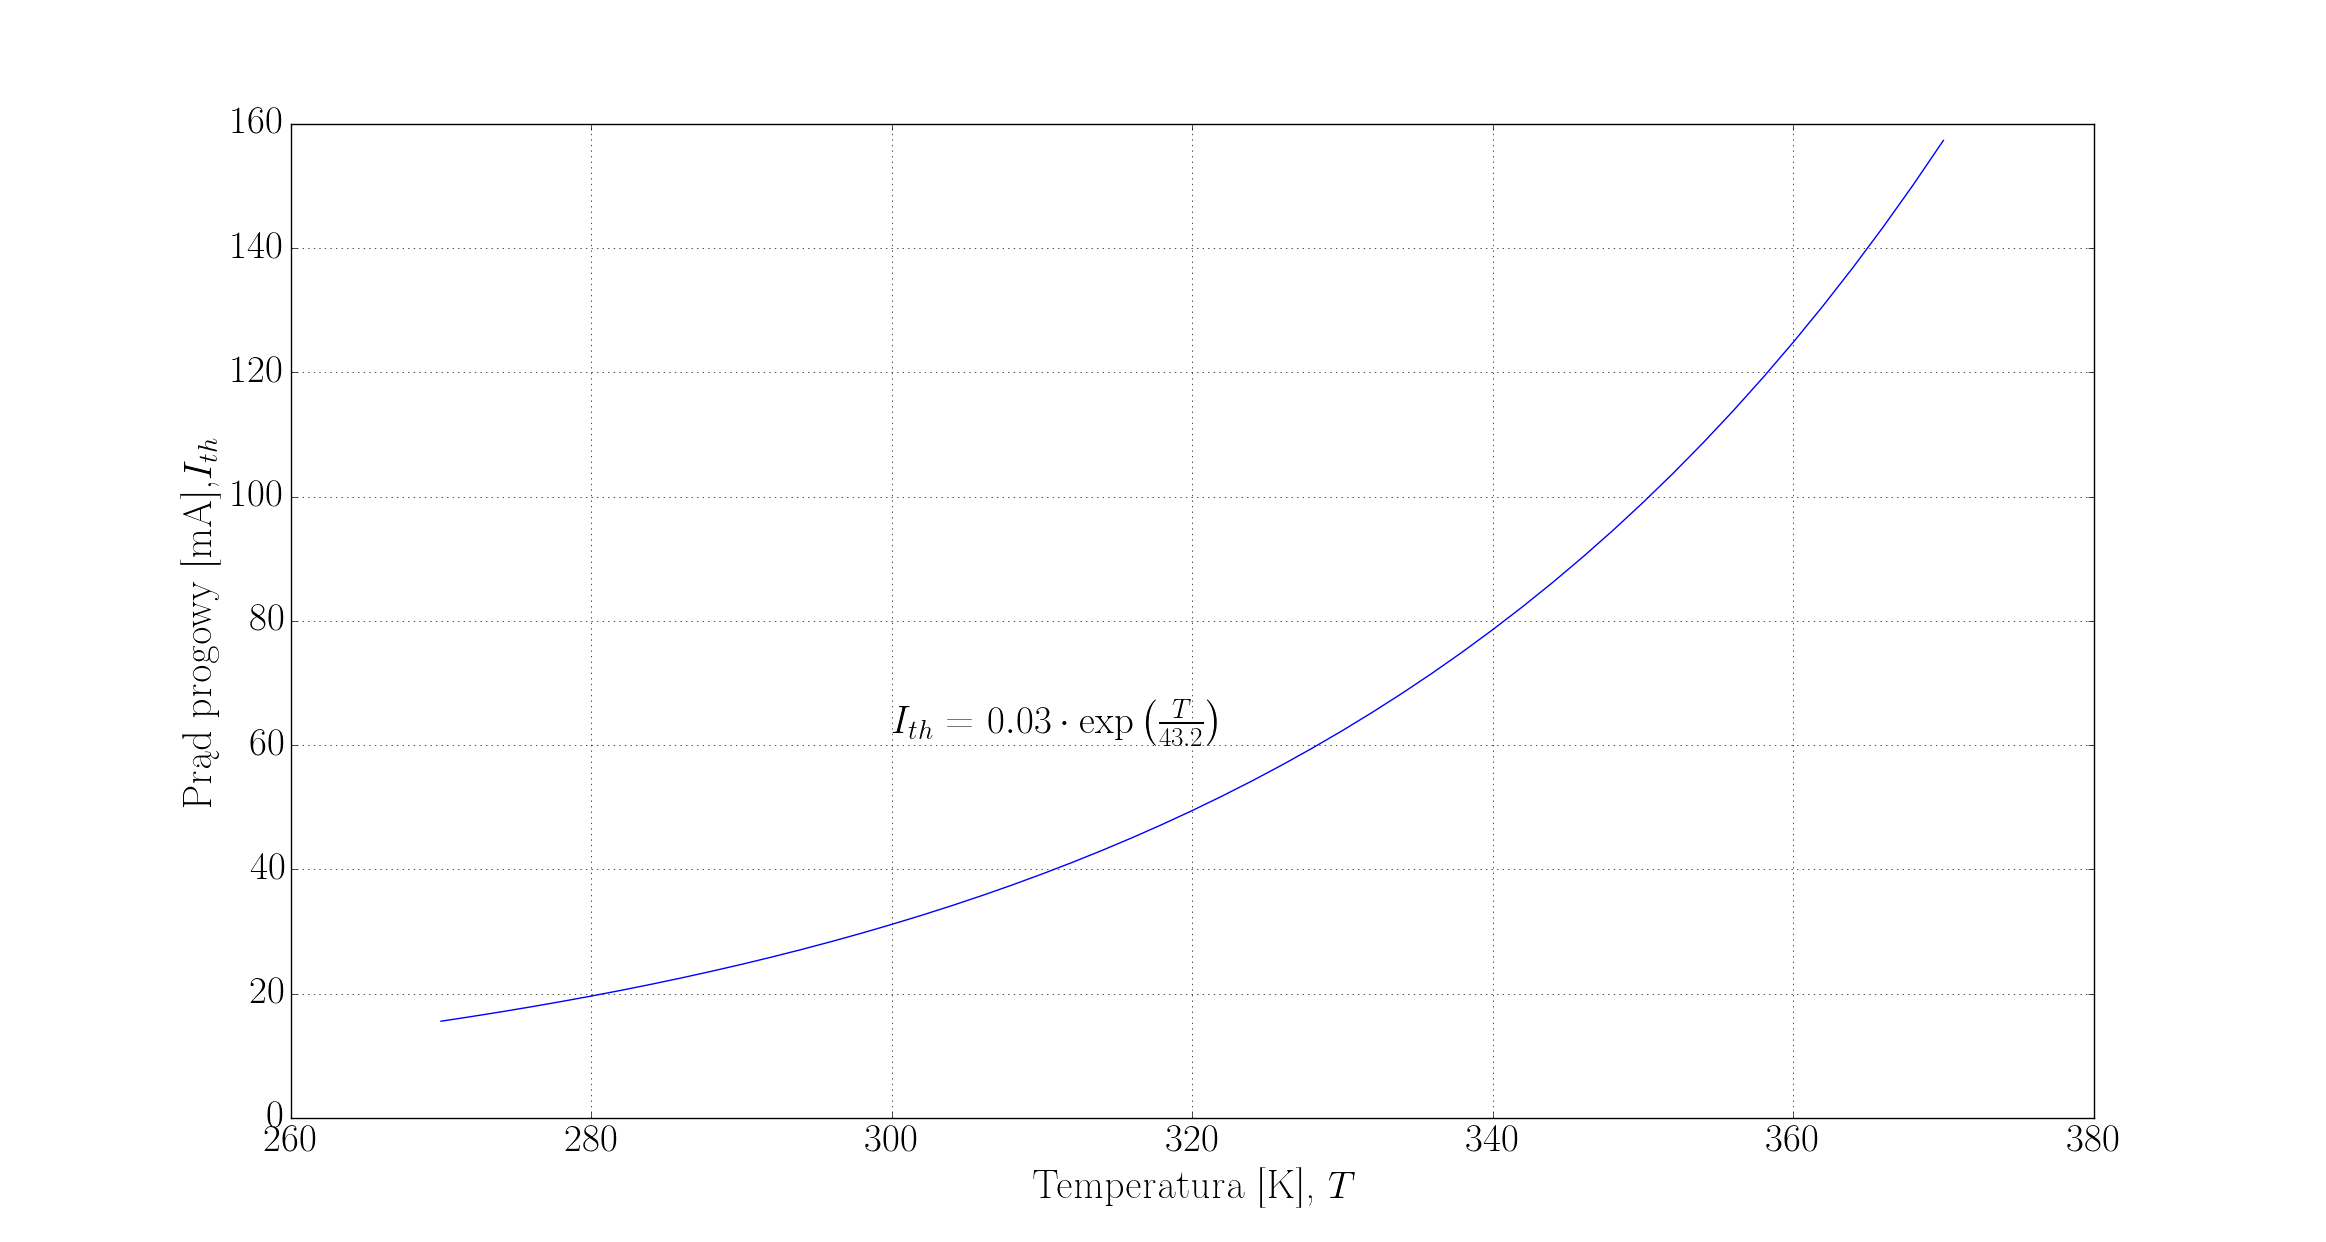
\includegraphics[width=1.10\textwidth,natwidth=69,natheight=87]{635/plot_i_th_temp.png}
\end{figure}
\end{frame}

\begin{frame}
\frametitle{Laser krawędziowy 635\,nm --- wykres mocy wejściowej do wyjściowej}
\center
\begin{figure}
%\hspace{4cm}  \vspace{1cm}
   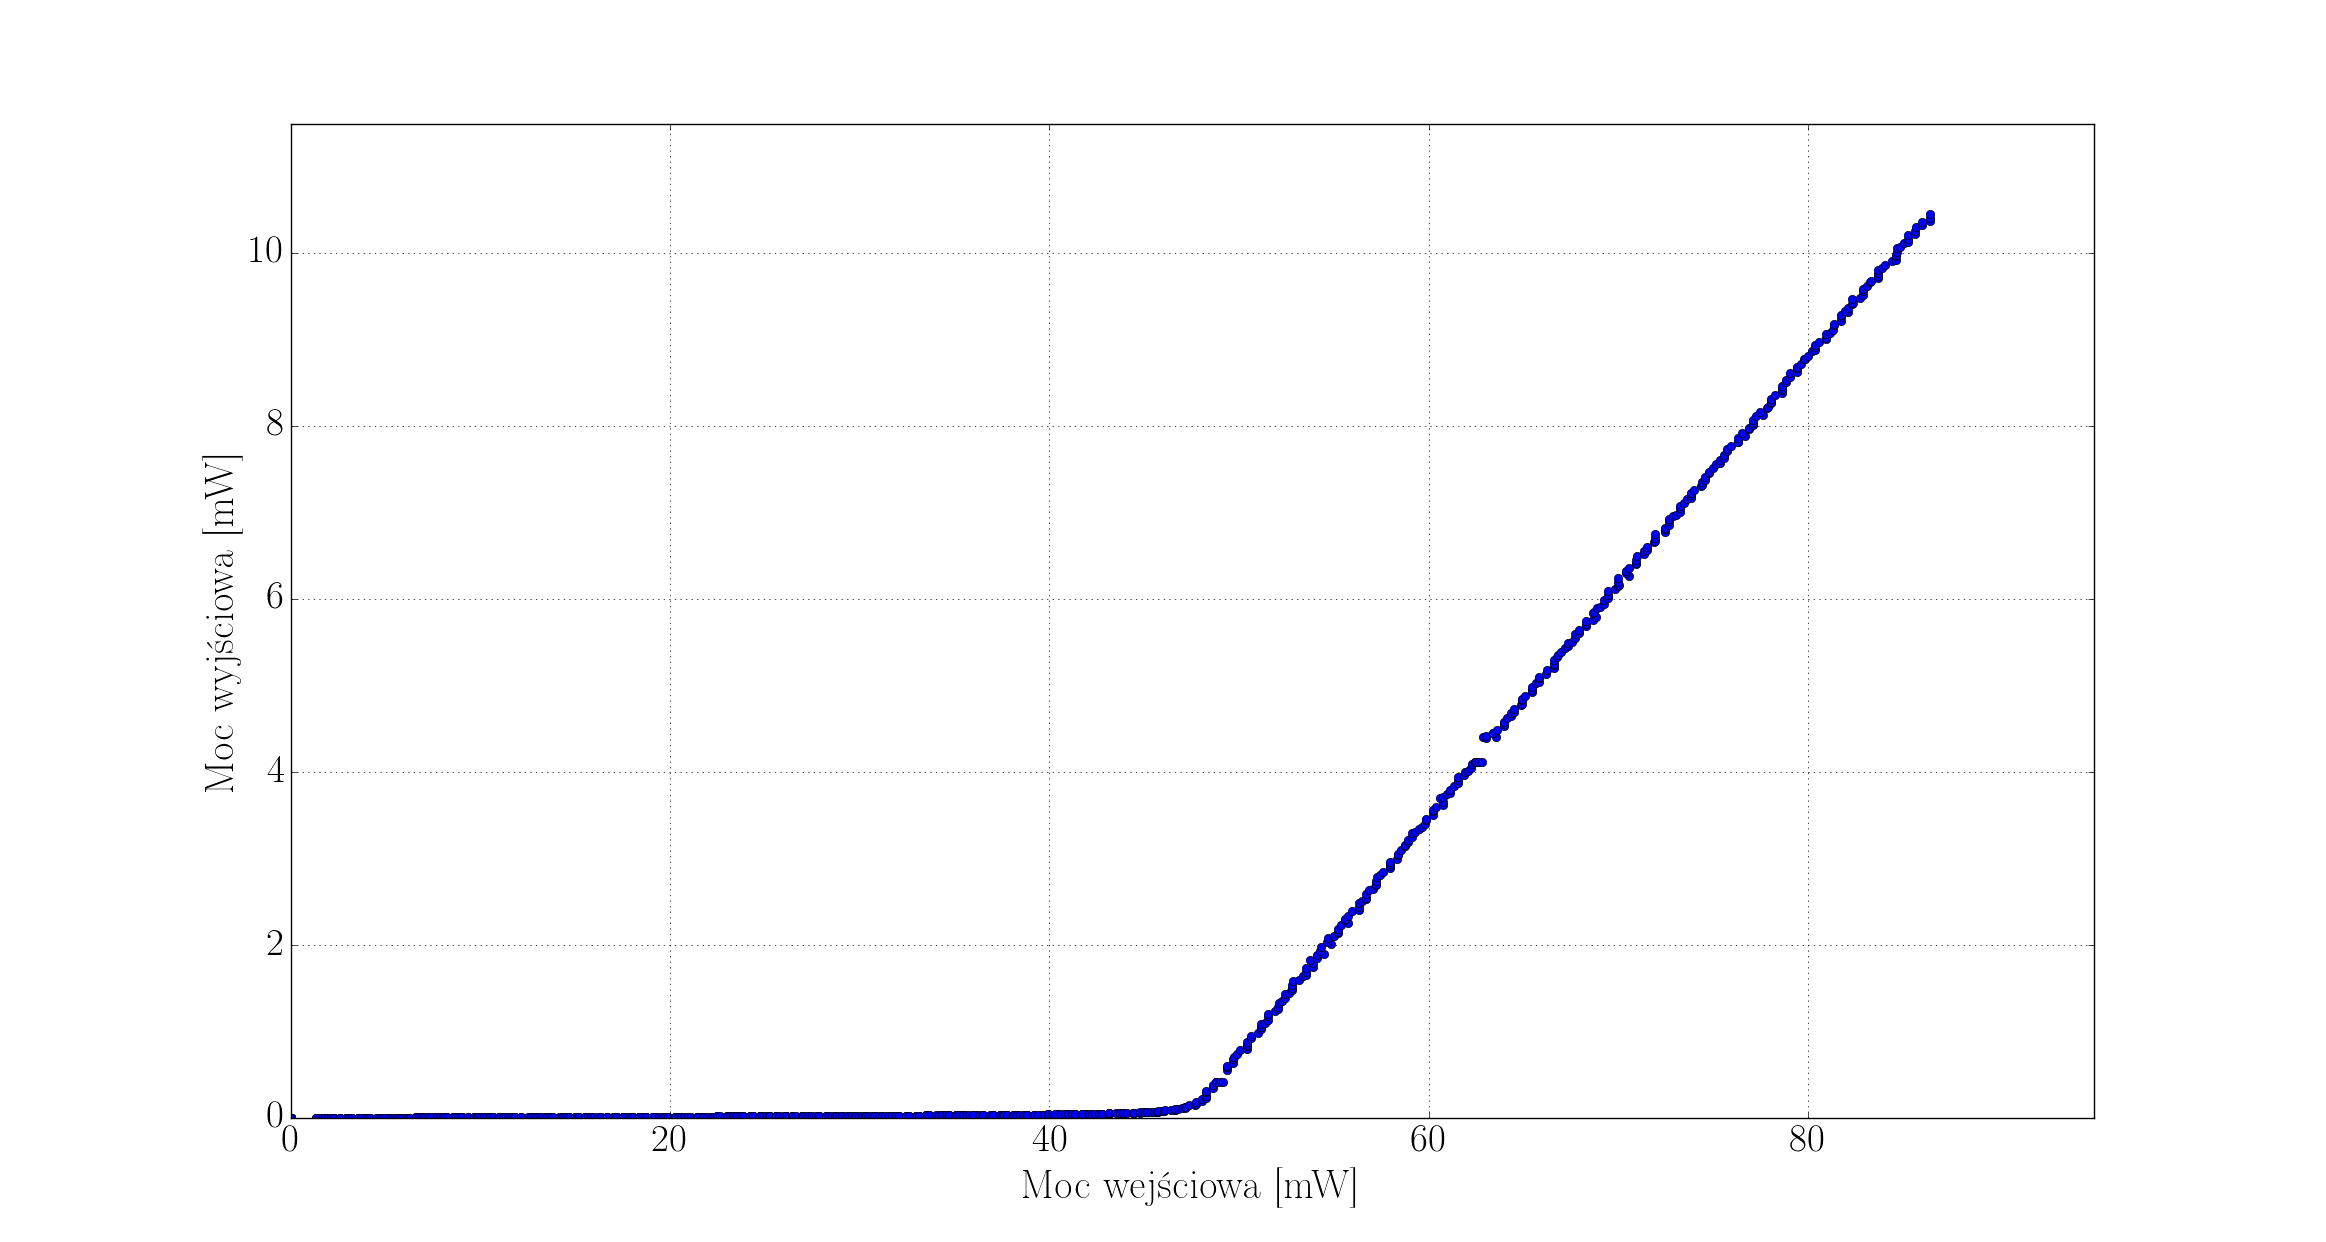
\includegraphics[width=1.10\textwidth,natwidth=69,natheight=87]{635/plot_power_20.png}
\end{figure}

\end{frame}

\begin{frame}
\begin{Huge}
\begin{center}
Podsumowanie
\end{center}
\end{Huge}
\end{frame}


\begin{frame}
\frametitle{Co dalej?}
\begin{itemize}
\item Wykoanie analiz innych laserów.
\item Rozbudowanie eksperymentu.
\end{itemize}
\end{frame}

\begin{frame}
\begin{Huge}
\begin{center}
Dziękueje za uwagę
\end{center}
\end{Huge}
\end{frame}

\begin{frame}
\begin{Huge}
\begin{center}
Pytania?
\end{center}
\end{Huge}
\end{frame}



\end{document}